

\chapter{Schematic Outlay Generation for Elements}
\label{sec:schematicoutlay}

%\begin{quotation}
%�Chaos in the world brings uneasiness, but it also allows the opportunity for creativity and growth.�
%\caption{Tom Barrett}
%\end{quatation}





%l-system uitleg hier 

I am interested in the structure of trees and the possibilities and restrictions it poses for placement of 
architectural shapes. For the purpose of this thesis the generated trees do not have to be visually convincing, however the basic shape should still be identified as a tree. The geometric properties of a tree model that are to interest of us are those that have effect on the possibilities with respect to the incorporation of architectural man-made structures. The tree geometry functions as the support structure for the building blocks I define in detail in section \ref{sec:treehousearch}. 

In this section we will discuss a method that generates a graph representing the structure of elements in a forest environment.  


\section{Scattering Techniques for Tree Positions}
\label{sec:scattering}

\section{Ecosystem Modeling}


\section{Multilayer TreeNode Generation}

%Previous plant ecosystem generation techniques were mainly focused at generating visually realistic con 

%todo: alter
For our method we have to be able to strategically place geometric architectural elements within tree structures. Finding the positions at which these architectural elements can be placed could be performed as a postprocess type process by analyzing the generated geometry, however we have the oppertunity to incorporate positional semantic information to the trees during the generation phase which simplifies the problem. 

L-system tree generation methods are mainly focused at producing convincing visual representations of trees \citep{Prezmyslaw}. However, we do believe that these methods can be extended quite easily to enable the addition of structural semantics. This thesis does not pursue the introduction of such an extension. For our problem we mainly have to deal with structure of a forest which we will abstract to a set of nodes, representing trees, for the moment. Finding useful connections between nodes and incorporation of structual elements within these tree nodes is what we are interested in.    

We propose a multilayer graphbased approach for the generation of a schematic outlay for elements in a forest structure. The nodes in this structure function as empty slots which define semantics that determine the type of elements this node can contain. See figure \ref{fig:treenodes} for an example element graph for a single tree.    

The element properties of a node are used to query the architectural element database. Listing \ref{list:properties} shows an example of element properties for a node. 

\lstset{language=Java, caption=Example of node element properties, label=list:properties, basicstyle=\footnotesize,
frame=shadowbox, rulesepcolor=\color{black}}

\newpage

\begin{lstlisting}

Element_node_14
{
	single_node_platform
	{
		available = true; 
		max_diameter = 30.0;
	}
	
	bridge
	{
		available = false; 
		type = suspension;
	}
	
	multi_node_platform
	{
		available = true; 
		other_nodes = array{34, 23, 78};
		type = undefined;
	
	 if (used)
	 		bridge.available = true;
	 else
	 		bridge.available = false; 		
	
	} 
	
	building
	{
		available = false;
	}
	
	stairs
	{	//staircase connection to parent node
		available = true; 
		type= revolving; 
	}
}

\end{lstlisting}

I will cover node element properties and quering of the element database in the next chapter in more detail.   

%The global forest schematic consists of a set of tree element schematics which have been scattered on a plane using the scattering technique discussed in the %previous section. The schematic of the forest includes all possible connections (bridges) between element graphs. Nodes in an element graph of a tree are contained %in a layer that contains the nodes positioned at the same height in all trees of the forest. The number of layers is determined by the element graph with highest %node level.  

%The height ($z$ coordinate) of a node is determined by the height property of the containing layer, while the position of a node in the plane defined by the layer %represents the $x,y$ coordinate of the branch.  

Our schematic outlay generation method uses the following parameters: 

\begin{enumerate}
\item Area  $A$  
\item Density $D (0.0 < D < 1.0)$  
\item Layers $L (L > 0)$ 
\item Tree parameters defining min bounds $T_{min}$
\item Tree parameters defining max bounds $T_{max}$
\item LocalTreeDeviation (controls deviation of tree properties within an area of size ClusterArea)
\item ClusterArea
%\item GlobalTreeDeviation
\end{enumerate}

%quick overview
With these parameters in place I can start discussing the algorithm. The rootnodes of our tree element graphs are contained by the base layer. The algorithm start by assigning 2d coordinates to the root nodes of each element graph using the scattering algorithm.

The scattering algorithm requires the $Area$, $Density$ parameters and the bounding $Tree parameters$ which determine the actionradius for
the generated trees. For each root node the algorithm sets a semi-random parameterset $P_t$ ($T_{min} < P_t < T_{max}$). The second step of the algorithm creates the upper $L-1$ layers. 

A layer is in fact a container for element nodes of all trees that allow connections through bridging. Nodes within a single layer roughly have the same height to the baselayer. Whether two nodes within a layer can be connected with a direct bridge depends on the element element properties of these nodes, the distance between them, and obstructions caused by other nodes.   

With the layers in place we iterate through the root node list in the base layer. For each root node a corresponding element graph is build. The method that builds an element graph depends on the global parameters of the forest but also on the structure of local neighbours. The method performs local statistical analysis on local element graphs within an area of size $ClusterArea$, and the result, combined with the $LocalTreeDeviation$ parameter, is used to generate a deviating tree element graph. Again note that the nodes in the element graph provide information about allowed architectural elements at this node, and the edges of an element graph represent connections by means of stairs or bridges. The element graph is in fact a subgraph of the final tree-structure graph that I will discuss in section \ref{sec:ElementToTree}.    

Growing an element graph for a tree means iterating through the layers. For each layer, $n$ ($0>= n >MaxNodes$) nodes with element properties are generated (a pointer to each node is stored in the local tree element graph and the corresponding layer). Note that when the element graph has no nodes at a specific layer this does not mean that the graph has stopped growing. Instead it means that the final tree structure prohibits elements to be placed at this position. When a new node is added to a layer the method tries to connect it to local nodes, provided that the node allows bridge connections. Figure \ref{fig:layers} shows a configuration of element graphs.

\begin{figure}[h]
	\centering
		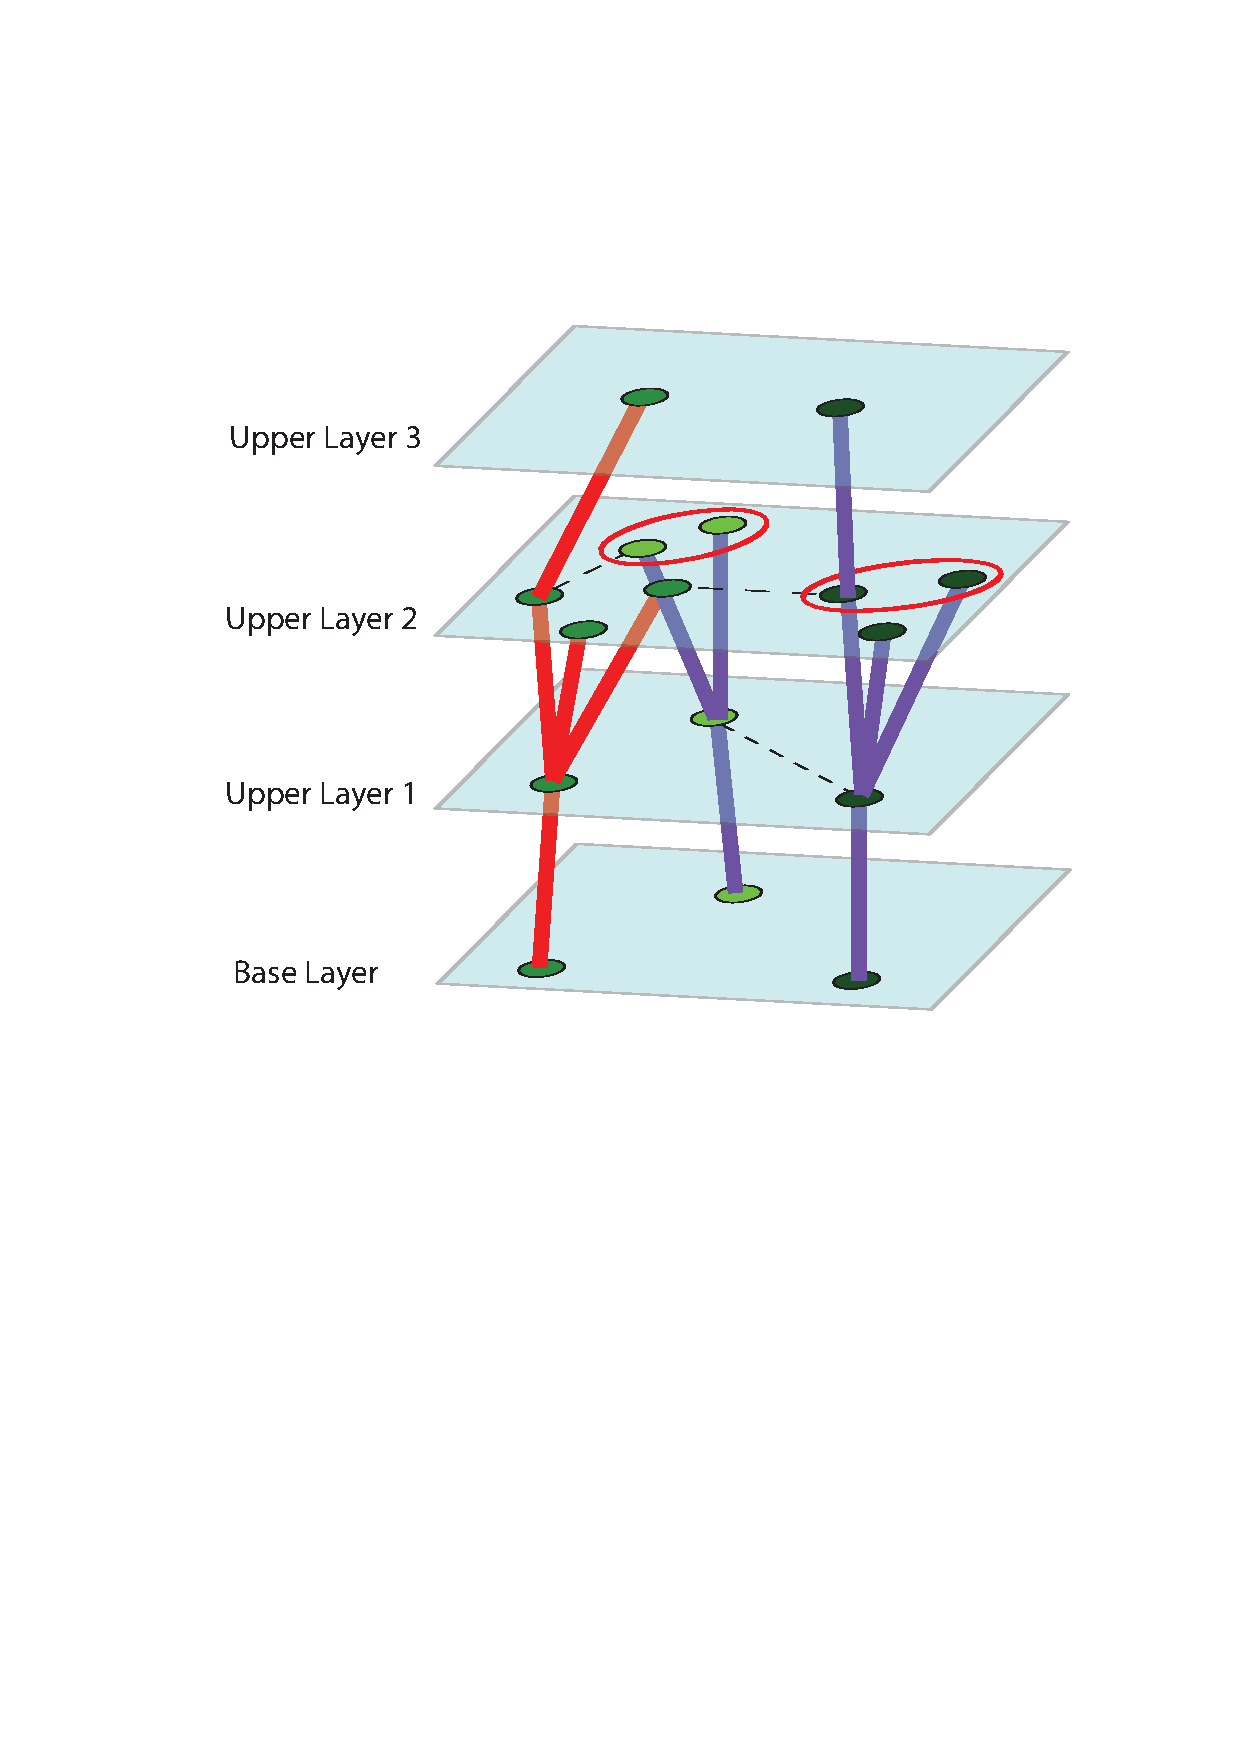
\includegraphics[width=220px]{images/element_graph_layers.pdf}
	\caption{example of multilayer element graphs for a small tree set}
	\label{fig:layers_and_graphs}
\end{figure}

When all element nodes have been constructed and placed into corresponding tree element graphs and layer element graphs the method checks wether all nodes are reachable from any other nodes. Single nodes or sets of connected nodes that are not reachable from the the main node graph will be deleted. We now have the schematic structure of a forest which we need as input for the architecture planning method discussed in the next section.          

% For every node $n_i$ contained by the base layer the method performs the folowing steps:  

%\begin{enumerate}
%\item Step1: 
%\item Step2:
%\item Step3:
%\item Step4:
%\end{enumerate}


%%%%%


%wat moet er nog in:


%- geven we de boom met een aparte node weer?	
%- wat nou als een platform support wordt door meerdere bomen -> meerdere nodes 
%		mogelijke oplossing: als een set van nodes een platform ondersteund, deze nodes als 1 node 
%   behandelen, dus zijn er twee graphs nodig. 1 voor alle nodes, 2e voor graph waarin bepaalde platformnodes samen worden gevoegd tot 1 node.   
 
%- hoe wordt een boom graph opgebouwd?
%- per upper layer is er voor elke branch een bounding area waar het in terecht kan komen
%- vaststellen van mogelijke connecties (bruggen) 
%- proces volgorde: eerst bepalen welke elementen we willen kunnen plaatsen in de boom
%- hoe beschrijft de semantiek welke elementen kunnen worden geplaatst? 

\newpage
\subsection{Simple Tree Structure}

Procedurally generating trees by means of l-systems has had a great amount of succes since the original proposal by Lindenmayer. The L-system formalism is widely applied in  academic work and is also succesfully used within commercial applications. This thesis does not focus on the l-system formalism in particular, since it is already a well established theory \citet{PrzemyslawAlgoBeauty}. I describe L-system in short in the following section as it is the most used fomalism for the contruction of trees.  


\subsection{Creating Tree Geometry}



 
%%%%%%%%%%%%%%%%%%%




%%%%%%%%%%%%%%%%%%%






%After construction of the multilayer graph representation of the forest, we feed it to the architecture planning algorithm that is discussed in section %\ref{sec:architecture}. 



%calculation of interval here     

%The first step of the method involves creation of $n$ ($0 <n < MAX_LAYERS$) layers.          
%The trunk node of every tree is placed inside the base layer.
%We will eventually translate the node based configuration of a forest to a visual representation   
%Therefore we propose an alternative method for the generation of forests as previous forest generation %methods do not incorporate semantic information  
%We propose an alternative method for the generation of forest geometry which supports    
